\documentclass[11pt,a4paper,onecolumn,draft,titlepage]{article}
\usepackage[utf8]{inputenc}
\usepackage{amsmath}
\usepackage{amsfonts}
\usepackage{amssymb}
\usepackage{graphicx}
\usepackage{ulem}
\author{Nico Andrew Glas}
\title{Diage: A Dialogue Generator}

\newcommand{\code}[1]{\texttt{#1}} %layout of game titles
\newcommand{\diage}{\textsl{Diage }}
\makeatletter

\makeatother

\makeindex
\begin{document}
\maketitle
\section*{Abstract}
When we create games, much of our time goes in to story writing (where applicable), and while this is unavoidable in narrative heavy games, we can automate it for 'non-critical' dialogue. For example, in the Pokémon RPGs the player can speak to every NPC in the game. All of these monologues were written by a story writer, even the singular sentences that hold no value to plot. We believe that with the right tooling we can automate this process and save valuable development time. \cite{riedl04} \cite{riedl03}
\section*{Acknowledgements}
\Huge TODO
\newpage
\normalsize
\tableofcontents
\newpage
\section{Introduction}
\Huge TODO
\subsection{Create-IT}
\Huge TODO
\subsection{Problem definition}
\Huge TODO
\subsection{Related work}
\Huge TODO
\subsection{Proof of concept}
\Huge TODO
\section{Defining a story}
\normalsize In our setting the "story" is a collection of coherent events that move forward in time with definitive starting and ending positions. For example; We define our story to begin with our hero Jack in his house and he wants to go to Jill's house for reasons. We can hereby define our story's initial state as:
\begin{itemize}
\item[] \textsf{S}: Jack \textsc{in} Jack's House
\item[] \textsf{P}: Jack \textsc{in} Jill's House
\end{itemize}
In this case, the \textsf{P} is the last plot point in our story, thus it will become an Ending (notated as \textsf{E}). We want to be able to exercise a director's role in the system, e.g. being able to make sure some plots will play out, but we do not want to keep filling in on how this should be executed. That should be the actors responsibility. 

\section{Representing a story}
This section will cover the modelling language I use to visualize the flow of information, some static and some waiting for the interaction of the player to release this information and ensuring plot progression.

\begin{figure}
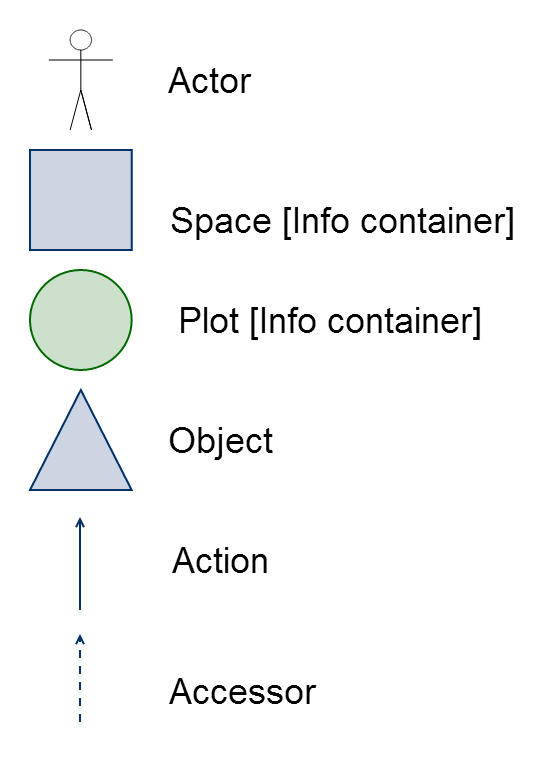
\includegraphics[scale=0.3]{img/symbols}
\caption{List of Declarative Symbols}
\label{fig:symbols}
\end{figure}
In figure~\ref{fig:symbols} we see the list of symbols that I use in the \\diage system\footnote{So, \\diage is becoming a modelling system as well? I really need to work on naming stuff.}. An actor can represent anything within the story that can, as the noun implies, act. Be that a store clerk, a brave adventurer or indeed the player himself. These actors have a knowledge pool that immediately conveys what he does and does not know.
Spaces represent world spaces such as; rooms, buildings and complete worlds. They are also defined as information containers. This means that spaces have information that will be shared with an actor the moment said actor steps into the space. For example, as the player walks in to a new town, his actor representation will know where the local store is. This information sharing is limited to other spaces within the parent space. So in the aforementioned example the player would know that there is a local store, but he doesn't know what that store sells, as that is a different entity.
Plots on the other hand are volatile information containers that release information on completion. Plots are also actions that the player must do to get plot progression. This does not mean that every plot should be mandatory, but without it some information will never become available. Plots, just like spaces, are nestable. When this happens, a plot turns in to a side-story which should - as the main story - have a definitive start and end position for the player.
Objects are rather straight-forward. In the local store from previous examples we could have the desk, an apple or a new sword. The only items that should be represented in \diage should be those that have a plot importance. Think of them as Checkov's guns, if you will~\footnote{A trite to smug, mayhaps? But I do like the idea of making \\diage using a strict literary vernacular}.
Actions define what actors can do with something or some one and accessors declare what actors know about a given subject. The latter is commonly used in conjunction with plots, signifying an increase in knowledge the moment that said plot is resolved. When incorporated in a full diagram we get something like figure~\ref{fig:diagram1}. An other form of notation used is shown in figure~\ref{fig:swimlane}. This is less verbose and therefore has less detail, but gives more oversight. These diagrams are called swimlanes~\footnote{Aw, hell no. Swimlanes? Come on, you can do better} and should remain static and does not contain any dynamic information. These could be seen as the \textit{status quo} for a given space. More research is needed to make a definitive conclusion on a sensible and readable notation.
\begin{figure}
\label{fig:diagram1}
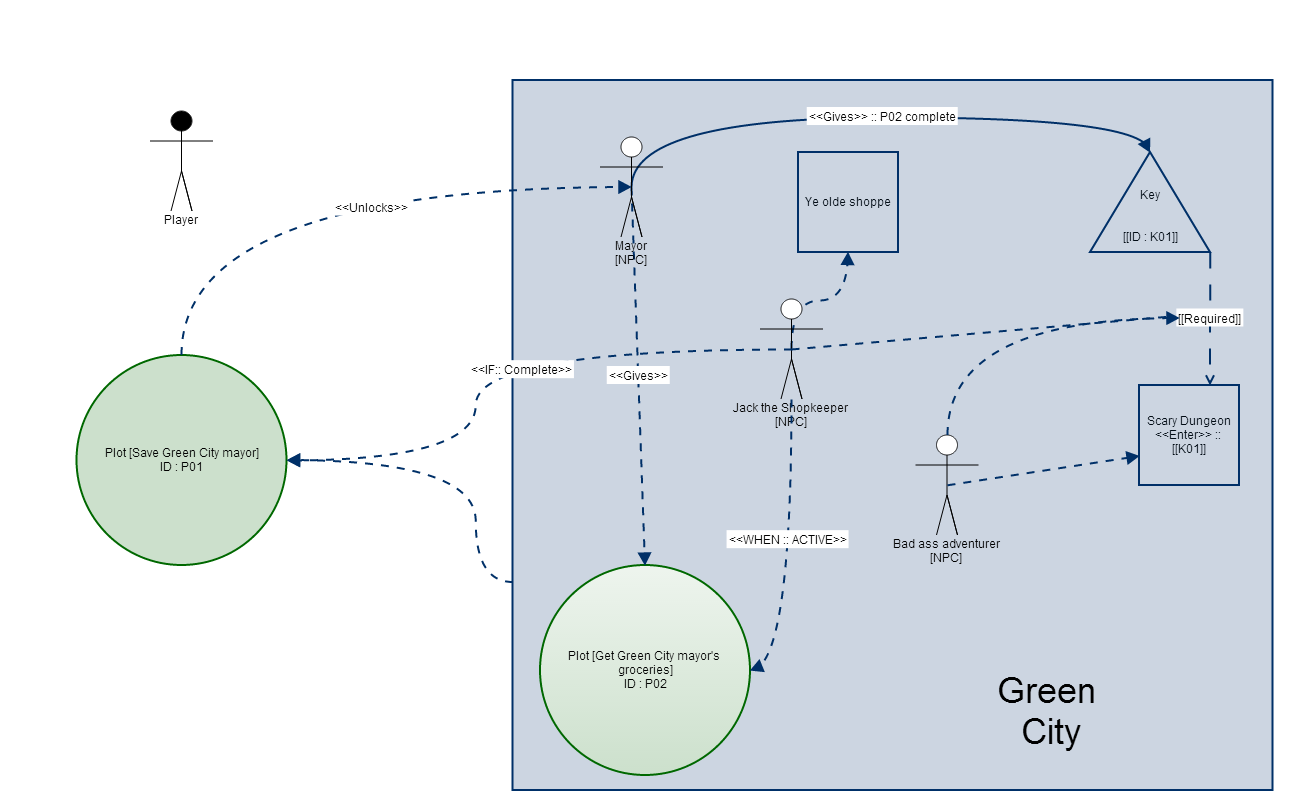
\includegraphics[scale=0.3]{img/diagram_example_1}
\caption{A \diage Diagram}
\end{figure}
\begin{figure}
\label{fig:swimlane}
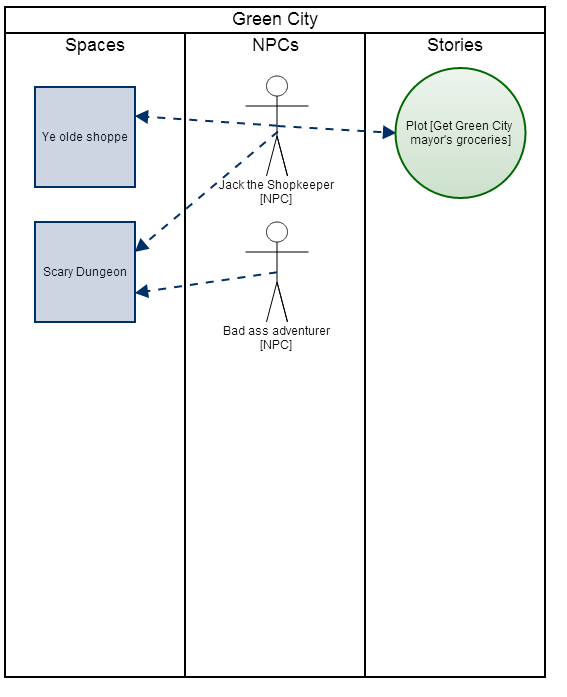
\includegraphics[scale=0.5]{img/swimlanes}
\caption{\diage swim lane diagram}
\end{figure}
\section{Usage in Ludoscope}
\Huge TODO
\section{Further study}
\label{sec:further_study}
\Huge TODO
\normalsize	
\bibliographystyle{plain}
\bibliography{diage}
\end{document}